\subsection{Позициониране чрез независими източници}

В източник \cite{bristolBeacons} се описва пасивна система [фиг. \ref{bristolVis}], в която движещ се обект използва ултразвукови сигнали от няколко източника, за да определи позицията си в пространството. Движещия се обект използва разликите в периода на сигнала, което е форма на Доплеров ефект, за да определи своята позиция и скоростта си. Този подход е нов и се счита за иновативен в измерването на разстоянието между различните обекти. Различава се от стандартния подход наречен time of flight (TOF). Използвания подход от хардуера, който е използван в текущата разработка е специфициран като радио честота и ултразвук \cite{hexamite} (спецификацията на апаратите не е публикувана). Съществуват и други разработки за измерване на разстоянието пример, за което е \cite{fastAndAccurate}, в който е демонстрирано използването на "phase accordance method". В източник \cite{bristolBeacons} чрез използване на измервания на периода на получаване на сигнали, системата успешно идентифицира източника на даден сигнал. За да се гарантира, че приемника правилно ще идентифицира кой е текущия трансмитер, се използват подбрани периоди така че да не се получават конфликтни идентификации. За всеки трансмитер се изчислява, каква е промяната през изминалия период с помощта на зависимостта, която гласи, че изменението на пулса е пропорционално на разстоянието, което получателя е изминал през дадения период. Тази зависимост се изразява в израз \ref{prop}.

\begin{figure}
    \centering
    \centerline{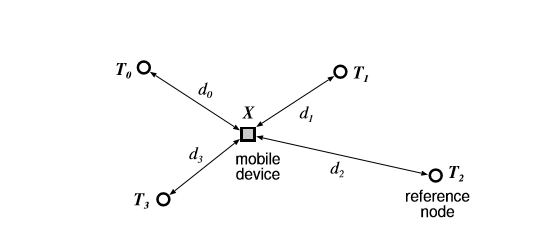
\includegraphics{bristolConfig}}
    \caption{Конфигурация на трансмитери и получатели}
    \label{bristolVis}
\end{figure}


\centerline{\begin{equation} \label{prop}
    \Delta d = v_s \Delta P_i
\end{equation}} \\

Системата се нуждае от поне 7 трансмитера, за да работи коректно.

За да се определи позицията на обекта се използва Калман филтър с множество хипотези \cite{kalmanFilter}. За да се определи позицията се използва формула \ref{kalman}.

\centerline{\begin{equation} \label{kalman}
    ((X-T_i)/ (|X-T_i|)) * V = (\Delta P_i * v_s) / (P_i + \Delta P_i)
\end{equation}}\\

Чрез изпълняване на много паралелни филтри се генерират хипотези за позицията на обекта в пространството. След протичането на този процес хипотезите се комбинират. В източник \cite{bristolBeacons} е решено хипотезите да бъдат комбинирани чрез усредняване на координатите. \\


\strong{Резултати} \\
Чрез използване на Калман филтър са измерени резултатите изобразени на фиг. \ref{fig:bristolResults}

\begin{figure}
    \centering
    \centerline{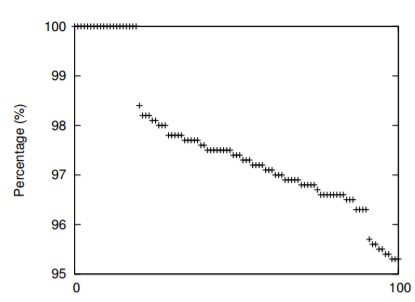
\includegraphics{bristolResults}}
    \caption{Качество на резултатите в проценти, при низходящо сортирани по дистанция данни}
    \label{fig:bristolResults}
\end{figure}